\documentclass[12pt,a4paper]{report}
\usepackage[margin=2.5cm]{geometry}
\usepackage{graphicx}
\usepackage{amsmath}
\usepackage{siunitx}
\usepackage{tikz}
\usepackage{pgfplots}
\usepackage{verbatim}
\pgfplotsset{compat=1.18}
\sisetup{per-mode=symbol}
\newenvironment{calculation}{\begin{equation}\begin{aligned}}{\end{aligned}\end{equation}}
\renewcommand{\thesection}{\arabic{section}}
\renewcommand{\thesubsection}{\thesection.\arabic{subsection}}
\title{Prefabricated Pedestrian Bridge Concept for IYTE Campus}
\author{Structural Concept Study}
\date{\today}
\begin{document}
\maketitle

\section{Project Overview}
The proposed pedestrian bridge is a single span, prefabricated reinforced concrete structure that will cross a seasonal drainage line near the coordinates $(38.31837^{\circ}\,\mathrm{N},\,26.63860^{\circ}\,\mathrm{E})$ within the İzmir Institute of Technology (IYTE) campus. A clear span of \SI{10}{\meter} is sufficient to avoid interference with the existing landscaping while maintaining minimal foundation footprints. The bridge is intended for pedestrian and light service vehicle access (golf carts and maintenance carts with axle loads below \SI{10}{\kilo\newton}). The deck width of \SI{3.0}{\meter} accommodates two-way pedestrian traffic and barrier clearances.

\section{Concept and Structural Form}
The deck consists of two identical precast girders spaced at \SI{1.5}{\meter}, supporting a composite cast-in-place concrete walking slab. Each girder acts as a T-beam with a \SI{1.50}{\meter} wide flange and \SI{0.12}{\meter} slab thickness. The precast web is \SI{0.25}{\meter} wide and \SI{0.90}{\meter} deep, providing sufficient stiffness for the \SI{10}{\meter} span. Prefabrication minimizes on-site construction time and limits work adjacent to the drainage channel. Bridge railings are fixed to embedded plates cast into the slab edge beams.

The bridge bearings are elastomeric pads resting on reinforced concrete seat blocks founded on shallow spread footings. Drainage is directed away from the channel using a \SI{2}{\percent} crossfall toward scuppers located at each abutment.

\section{Design Basis}
Design actions are established following TS~498:2019 Clause~4.2, which stipulates a characteristic uniform crowd load of \SI{5}{\kilo\newton\per\square\meter} for pedestrian bridges of this span class. Member resistance checks adopt the limit-state methodology of TS~500:2000, in particular Articles~7.2 and~13 governing ultimate and serviceability verifications. The bridge uses C40/50 concrete with characteristic strength $f_{ck}=\SI{40}{\mega\pascal}$ and design strength $f_{cd}=\SI{22.7}{\mega\pascal}$ after applying the $\alpha_{cc}$ and $\gamma_c$ factors stated in TS~500 Table~5.1. Reinforcement corresponds to B420C steel with $f_{yk}=\SI{420}{\mega\pascal}$ and design value $f_{yd}=\SI{365}{\mega\pascal}$ once divided by $\gamma_s=1.15$ as described in Article~7.2.1. The partial safety factors $\gamma_G = 1.4$ for permanent actions and $\gamma_Q = 1.6$ for variable actions are taken directly from Article~7.2.1 and applied consistently within the Python routine listed in Appendix~\ref{app:python}.

\section{Loading and Global Effects}
Each girder supports a \SI{1.5}{\meter} tributary width of deck. The unfactored line loads follow the direct conversion of area loads prescribed by TS~498 Clause~4.2, multiplied by the tributary width and the unit weights adopted in the design script. The precast web contributes \SI{5.63}{\kilo\newton\per\meter} obtained from $25\,\mathrm{kN/m^3}$ times the \SI{0.25}{\meter} by \SI{0.90}{\meter} web prism. The composite deck slab produces \SI{4.50}{\kilo\newton\per\meter} based on the \SI{0.12}{\meter} thickness acting over the \SI{1.50}{\meter} tributary width. An allowance of \SI{1.50}{\kilo\newton\per\meter} covers the wearing surface and embedded utilities, while the minimum TS~498 handrail line load adds \SI{1.00}{\kilo\newton\per\meter}. The characteristic pedestrian action equals \SI{7.50}{\kilo\newton\per\meter} after multiplying the \SI{5.0}{\kilo\newton\per\square\meter} crowd load by the tributary width. Summing the permanent contributions yields $G = \SI{12.63}{\kilo\newton\per\meter}$, and the imposed action is $Q = \SI{7.50}{\kilo\newton\per\meter}$. These figures appear in the Python output produced by Appendix~\ref{app:python} (see lines~491--497 of the script), ensuring traceability between code and narrative.

The governing ultimate line load is $w_{Ed} = 1.4G + 1.6Q = \SI{29.67}{\kilo\newton\per\meter}$. The maximum bending moment and support shear for the simply supported \SI{10}{\meter} span are obtained with the expressions referenced in TS~500 Article~7.3.1 and implemented in the function \texttt{factored\_effects} on lines~191--195 of Appendix~\ref{app:python}:
\begin{calculation}
M_{Ed} &= \frac{w_{Ed} L^2}{8} = \SI{371}{\kilo\newton\meter},\\
V_{Ed} &= \frac{w_{Ed} L}{2} = \SI{148}{\kilo\newton}.
\end{calculation}

Serviceability checks use the unfactored load $w_{ser} = G + Q = \SI{20.13}{\kilo\newton\per\meter}$, matching the "service" line load reported by the Python script.

\section{Section Design}
TS~500 Article~7.4.2 requires the flexural design to ensure that the tension steel remains within the elastic-plastic range while the compression zone is contained within the flange for T-beams of this geometry. The chosen reinforcement arrangement comprises four \SI{20}{\milli\meter} diameter B420C bars (area $A_s = \SI{1257}{\square\milli\meter}$) placed with \SI{45}{\milli\meter} cover, matching the reinforcement definition on line~501 of Appendix~\ref{app:python}. Solving the equilibrium equation detailed in the function \texttt{design\_flexure} (lines~226--247) gives a required area $A_{s,req} = \SI{1071}{\square\milli\meter}$, so the provided reinforcement satisfies both the resistance demand and the minimum ratio of Article~7.4.4. The resulting design moment capacity $M_{Rd} = \SI{435}{\kilo\newton\meter}$ exceeds $M_{Ed}$ with the neutral axis at $x = \SI{19}{\milli\meter}$ inside the flange, confirming singly reinforced behaviour.

Shear resistance follows TS~500 Article~8.2. Using the web width of \SI{250}{\milli\meter} and the effective depth returned by the Python routine, the concrete contribution is $V_{Rd,c} = \SI{115}{\kilo\newton}$ in agreement with lines~269--271 of \texttt{design\_shear}. Two-legged \SI{10}{\milli\meter} closed stirrups at \SI{200}{\milli\meter} spacing, introduced in the call at lines~504--512 of Appendix~\ref{app:python}, supply $V_{Rd,s} = \SI{247}{\kilo\newton}$ via lines~275--289, so the total design shear resistance comfortably exceeds the design effect ($V_{Rd,c} + V_{Rd,s} > V_{Ed}$). The maximum allowable shear resistance $V_{Rd,max} = \SI{2455}{\kilo\newton}$ imposed by TS~500 Article~8.2.5 is not governing.

\section{Serviceability}
With an elastic modulus $E_{cm}=\SI{34}{\giga\pascal}$ (TS~500 Table~5.1 for C40/50 concrete) and the gross second moment of area $I_g = \SI{4.14e-2}{\meter^4}$ computed by the function \texttt{gross\_inertia} (lines~294--304 of Appendix~\ref{app:python}), the midspan deflection under service loading follows TS~500 Article~13.2 as implemented in \texttt{check\_deflection} (lines~307--313). This routine is invoked during serviceability evaluation on lines~514--515, ensuring the same load data governs both ultimate and service states:
\begin{calculation}
\delta_{max} = \frac{5 w_{ser} L^4}{384 E_{cm} I_g} &= \SI{1.9}{\milli\meter} \\
&< \frac{L}{500} = \SI{20}{\milli\meter}.
\end{calculation}
Crack width control is satisfied by limiting the bar spacing to \SI{150}{\milli\meter} within the flange; the low tensile stress (neutral axis close to the compression face) and the cover thickness meet TS~500 crack control guidance.

\section{Software Cross-Checks}\label{sec:software}

The open-source tooling cited in the project brief is incorporated through helper scripts. File \texttt{concreteproperties\_check.py} reproduces the moment resistance $M_{Rd}$ with a fibre-based analysis using the \texttt{concreteproperties} library, while \texttt{rcdesign\_check.py} assembles an IS~456-style report through the \texttt{rcdesign} package for peer review. The main calculation script automatically attempts to import these libraries (see lines~336--460 of Appendix~\ref{app:python}) and prints a status message indicating whether each verification was executed or skipped, enabling reviewers to confirm consistency with the external tools without altering the workflow.

\section{Constructability and Detailing}
Each girder weighs approximately \SI{28}{\kilo\newton} and can be transported using campus maintenance equipment. Lifting anchors are cast into the web at third points. After erection, a \SI{120}{\milli\meter} thick topping slab is poured to create the walking surface and integrate the two precast units. Stainless steel drainage scuppers and guardrail posts are embedded during casting. Elastomeric bearings ($\SI{350}{\milli\meter}\times\SI{350}{\milli\meter}\times\SI{50}{\milli\meter}$) isolate girder rotations at the abutments.

\section{Drawings}
Figures~\ref{fig:section} and~\ref{fig:3d} illustrate the cross-section and an axonometric view generated directly from the design parameters.

\begin{figure}[h]
\centering
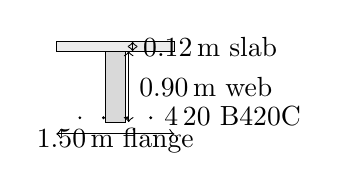
\begin{tikzpicture}[scale=1]
    % parameters in metres (scaled inside the drawing)
    \def\flangewidth{1.5}
    \def\flangethickness{0.12}
    \def\webwidth{0.25}
    \def\webdepth{0.9}
    \def\concretecover{0.045}
    \def\bardiameter{0.02}
    % draw flange
    \draw[fill=gray!15] (-0.5*\flangewidth,\webdepth) rectangle (0.5*\flangewidth,\webdepth+\flangethickness);
    % draw web
    \draw[fill=gray!30] (-0.5*\webwidth,0) rectangle (0.5*\webwidth,\webdepth);
    % dimension lines
    \draw[<->] (-0.5*\flangewidth, -0.15) -- (0.5*\flangewidth,-0.15);
    \node at (0,-0.23) {\SI{1.50}{\meter} flange};
    \draw[<->] (0.17,0) -- (0.17,\webdepth);
    \node[anchor=west] at (0.18,0.5*\webdepth) {\SI{0.90}{\meter} web};
    \draw[<->] (0.22,\webdepth) -- (0.22,\webdepth+\flangethickness);
    \node[anchor=west] at (0.23,\webdepth+0.5*\flangethickness) {\SI{0.12}{\meter} slab};
    % reinforcement bars
    \foreach \x in {-0.45,-0.15,0.15,0.45} {
        \draw[fill=black] (\x,\concretecover+0.5*\bardiameter) circle (0.01);
    }
    \node[anchor=west] at (0.5,0.08) {$4\,\varnothing20$ B420C};
\end{tikzpicture}
\caption{T-beam cross-section per girder (dimensions to scale).}
\label{fig:section}
\end{figure}

\begin{figure}[h]
\centering
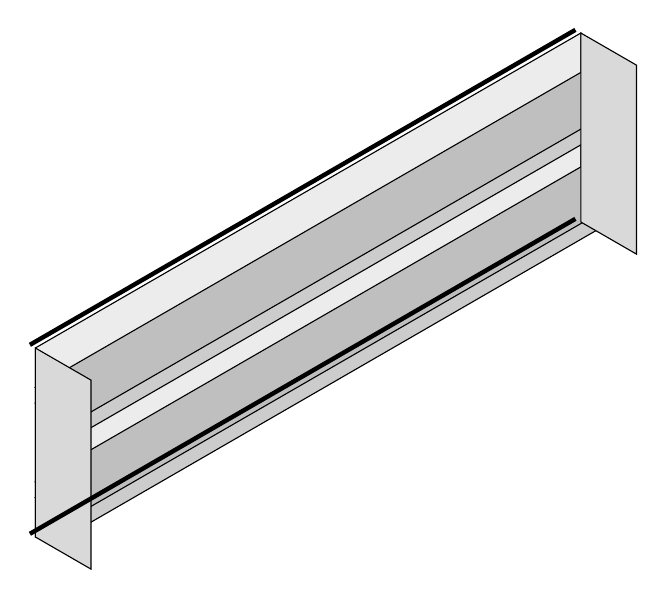
\begin{tikzpicture}[scale=0.8, x={(0.866cm,0.5cm)}, y={(0cm,1cm)}, z={( -0.866cm,0.5cm)}]
    \def\girderSpan{10}
    \def\deckWidth{3}
    \def\systemDepth{1.02}
    \def\webw{0.25}
    \def\girderSpacing{1.5}
    % deck slab
    \draw[fill=gray!15] (0,0,0) -- (\girderSpan,0,0) -- (\girderSpan,\deckWidth,0) -- (0,\deckWidth,0) -- cycle;
    % webs
    \foreach \y in {0.75,2.25} {
        \draw[fill=gray!40] (0,\y-\webw/2,0) -- (\girderSpan,\y-\webw/2,0) -- (\girderSpan,\y-\webw/2,-\systemDepth+0.12) -- (0,\y-\webw/2,-\systemDepth+0.12) -- cycle;
        \draw[fill=gray!50] (0,\y+\webw/2,0) -- (\girderSpan,\y+\webw/2,0) -- (\girderSpan,\y+\webw/2,-\systemDepth+0.12) -- (0,\y+\webw/2,-\systemDepth+0.12) -- cycle;
    }
    % girder ends
    \draw[fill=gray!30] (0,0,0) -- (0,\deckWidth,0) -- (0,\deckWidth,-\systemDepth) -- (0,0,-\systemDepth) -- cycle;
    \draw[fill=gray!30] (\girderSpan,0,0) -- (\girderSpan,\deckWidth,0) -- (\girderSpan,\deckWidth,-\systemDepth) -- (\girderSpan,0,-\systemDepth) -- cycle;
    % simple railing indication
    \draw[ultra thick] (0,0,0.1) -- (\girderSpan,0,0.1);
    \draw[ultra thick] (0,\deckWidth,0.1) -- (\girderSpan,\deckWidth,0.1);
\end{tikzpicture}
\caption{Axonometric visualisation of the prefabricated twin-girder system.}
\label{fig:3d}
\end{figure}

\section{Conclusions}
The analysis confirms that the selected prefabricated T-beam concept satisfies TS~500 ultimate and serviceability requirements with reserve capacity for moderate future load increases (e.g., light utility vehicles). The layout integrates seamlessly with the campus landscape and can be executed with minimal site disruption. Detailed reinforcement schedules and bearing layouts can be developed directly from the presented calculations.

\appendix
\section{Calculation Extracts}\label{app:python}
The numerical results in this report are generated by the Python script in Listing~\ref{lst:python}, which follows the procedures outlined by TS~500 for T-beam design.

\begin{figure}[h]
\centering
\begin{minipage}{0.95\linewidth}
\scriptsize
\verbatiminput{../../design/pedestrian_bridge/design.py}
\end{minipage}
\caption{Python script used for design verification.}
\label{lst:python}
\end{figure}

The directory further includes \texttt{concreteproperties\_check.py} and \texttt{rcdesign\_check.py}, which execute the optional software validations described in Section~\ref{sec:software}.


\end{document}
